\documentclass[11pt,a4paper]{article}

\usepackage[T1]{fontenc}
\usepackage[utf8]{inputenc}
\usepackage[margin=2.4cm, top=2.8cm, bottom=2.8cm, headheight=15pt]{geometry}
\usepackage{microtype}
\usepackage{xcolor}
\usepackage{booktabs}
\usepackage{tabularx}
\usepackage{multirow}
\usepackage{longtable}
\usepackage{array}
\usepackage{colortbl}
\usepackage{enumitem}
\usepackage{fancyhdr}
\usepackage{titlesec}
\usepackage{hyperref}
\usepackage{float}
\usepackage{caption}
\usepackage{tikz}
\usetikzlibrary{shapes.geometric, arrows.meta, positioning, fit, backgrounds, calc}

% ── Colour palette ───────────────────────────────────────────────────────────
\definecolor{primary}{HTML}{185FA5}
\definecolor{primarylight}{HTML}{E6F1FB}
\definecolor{teal}{HTML}{0F6E56}
\definecolor{teallight}{HTML}{E1F5EE}
\definecolor{purple}{HTML}{534AB7}
\definecolor{purplelight}{HTML}{EEEDFE}
\definecolor{amber}{HTML}{854F0B}
\definecolor{amberlight}{HTML}{FAEEDA}
\definecolor{coral}{HTML}{993C1D}
\definecolor{corallight}{HTML}{FAECE7}
\definecolor{rowgray}{HTML}{F7F6F2}
\definecolor{bordergray}{HTML}{DEDBD2}
\definecolor{textmuted}{HTML}{5F5E5A}

% ── Typography ───────────────────────────────────────────────────────────────
\usepackage{helvet}
\renewcommand{\familydefault}{\sfdefault}

% ── Section styling ──────────────────────────────────────────────────────────
\titleformat{\section}{\large\bfseries\color{primary}}{}{0em}{}[%
  \vspace{-4pt}\textcolor{bordergray}{\rule{\linewidth}{0.4pt}}]
\titleformat{\subsection}{\normalsize\bfseries\color{primary!80!black}}{}{0em}{}
\titleformat{\subsubsection}{\normalsize\itshape\color{textmuted}}{}{0em}{}
\titlespacing{\section}{0pt}{18pt}{8pt}
\titlespacing{\subsection}{0pt}{12pt}{4pt}

% ── Header / footer ──────────────────────────────────────────────────────────
\pagestyle{fancy}
\fancyhf{}
\fancyhead[L]{\small\color{textmuted}Warsaw Tram Delay Prediction Platform}
\fancyhead[R]{\small\color{textmuted}Architecture Report}
\fancyfoot[C]{\small\color{textmuted}\thepage}
\renewcommand{\headrulewidth}{0.4pt}
\renewcommand{\headrule}{%
  \hbox to\headwidth{\color{bordergray}\leaders\hrule height\headrulewidth\hfill}}

% ── Table helpers ─────────────────────────────────────────────────────────────
\newcolumntype{L}[1]{>{\raggedright\arraybackslash}p{#1}}
\newcolumntype{C}[1]{>{\centering\arraybackslash}p{#1}}
\newcommand{\hd}[1]{\textbf{\small #1}}
\newcommand{\ce}[1]{\small #1}

% ── TikZ styles ───────────────────────────────────────────────────────────────
\tikzset{
  svc/.style={rectangle, rounded corners=4pt, minimum width=3.0cm,
              minimum height=0.85cm, text centered,
              font=\small\bfseries, inner sep=6pt},
  ingestion/.style ={svc, fill=teallight,    draw=teal,       text=teal},
  processing/.style={svc, fill=primarylight, draw=primary,    text=primary},
  serving/.style   ={svc, fill=purplelight,  draw=purple,     text=purple},
  frontend/.style  ={svc, fill=corallight,   draw=coral,      text=coral},
  storage/.style   ={svc, fill=amberlight,   draw=amber,      text=amber},
  extapi/.style    ={svc, fill=rowgray,      draw=bordergray, text=textmuted},
  conn/.style={-Stealth, thick, color=bordergray},
  lbl/.style={font=\tiny\ttfamily, color=textmuted, fill=white,
              inner sep=1pt, midway},
}

% ── Hyperref ─────────────────────────────────────────────────────────────────
\hypersetup{colorlinks=true, linkcolor=primary, urlcolor=primary,
            pdftitle={Warsaw Tram Delay Prediction Platform}}

% ─────────────────────────────────────────────────────────────────────────────
\begin{document}

% ── Title page ───────────────────────────────────────────────────────────────
\begin{titlepage}
  \vspace*{2cm}
  \begin{center}
    {\LARGE\bfseries\color{primary}
      Warsaw Tram Delay Prediction Platform}\\[1.2cm]
    {\large\color{textmuted} Architecture Report}\\[0.4cm]
   {\large\bfseries Authors}\\[0.5cm]
    {\normalsize
      Wiktoria Koniecko \\
      Michał Szewczak \\
      Sebastian Trojan
    }\\[2.0cm]

    {\large \today}
  \end{center}
\end{titlepage}

\tableofcontents
\newpage

% =============================================================================
\section{System Overview}
% =============================================================================

The platform ingests three categories of data from the Warsaw city API
(\texttt{api.um.warszawa.pl}):

\begin{itemize}[itemsep=3pt]
  \item \textbf{Timetable data} (static, loaded once daily before 04:00) ---
    stop locations, line-stop assignments, and per-brigade precise schedules
    for every tram stop--line--brigade combination in the network.
  \item \textbf{Vehicle position data} (streaming, 04:00--01:00) --- live GPS
    pings for every active tram: \texttt{Lat}, \texttt{Lon}, \texttt{Time},
    \texttt{Lines}, \texttt{Brigade}, \texttt{VehicleNumber}.
  \item \textbf{Weather data} (periodic, throughout the day) --- temperature,
    precipitation, wind, and visibility for Warsaw.
\end{itemize}

The platform derives tram delays by matching live positions against the loaded
timetable, stores both raw and feature data in BigQuery, trains a delay
prediction model on Vertex AI, and serves two user-facing interfaces: a
real-time tram map with computed delays and a prediction UI.

The system scope is \textbf{trams only}. Operating window is
\textbf{04:00--01:00 daily} (21 hours). Outside this window no position data
arrives and all streaming components are idle.

% =============================================================================
\section{Timetable Loading Procedure}
\label{sec:timetable}
% =============================================================================

The timetable loader runs as a Cloud Run Job triggered by Cloud Scheduler at
\textbf{03:00 daily}, completing before tram service begins at 04:00. The
loading procedure is sequential and hierarchical:

\begin{enumerate}[itemsep=4pt]
  \item \textbf{Download all stops.}
    \texttt{GET /api/action/dbstore\_get} with the stops resource ID returns
    the full list of Warsaw tram stops: stop ID, stop number, stop name, lat,
    lon, direction.

  \item \textbf{For each stop: download all lines.}
    \texttt{GET /api/action/dbtimetable\_get} parameterised by stop ID returns
    the list of tram lines passing through that stop.

  \item \textbf{For each stop--line pair: download brigade schedules.}
    A further call to \texttt{dbtimetable\_get} parameterised by stop ID and
    line number returns all brigades serving that combination, together with
    precise scheduled departure times throughout the day.
\end{enumerate}

The result is a complete timetable: for every
(stop, line, brigade) triple the system knows the scheduled departure time at
every point in the day. This is the reference used by the Stream Processor to
compute \texttt{delay\_seconds} during operating hours.

\textbf{Volume estimate.} Warsaw has approximately 300 tram stops, 30 tram
lines, and on average 5--8 brigades per line per stop. The loader makes
roughly $300 + 300 \times 30 + 300 \times 30 \times 6 \approx 63\,000$
sequential API calls. At a conservative 200 ms per call this takes
$\approx$3.5 hours, which is too slow. The loader must therefore parallelise
the stop--line and stop--line--brigade calls using a bounded async pool
(20--50 concurrent requests), reducing wall-clock time to under 30 minutes.

% =============================================================================
\section{Microservice Map}
% =============================================================================

\subsection{Service inventory}

\begin{table}[H]
\centering
\caption{Microservice inventory}
\renewcommand{\arraystretch}{1.38}
\begin{tabularx}{\linewidth}{L{3.0cm} L{2.3cm} L{3.6cm} X}
\toprule
\hd{Service} & \hd{Runtime} & \hd{Responsibility} & \hd{Trigger / schedule} \\
\midrule
\rowcolor{rowgray}
\ce{Timetable Loader} & Cloud Run Job
  & Sequential--parallel download of stops, lines, brigades; write to BigQuery
  & Cloud Scheduler 03:00 daily \\
\ce{Position Ingestor} & Cloud Run Job
  & Poll tram positions every 60 s; publish to Pub/Sub
  & Cloud Scheduler every 60 s, 04:00--01:00 \\
\rowcolor{rowgray}
\ce{Weather Ingestor} & Cloud Run Job
  & Poll weather API; publish to Pub/Sub
  & Cloud Scheduler every 10 min \\
\ce{Stream Processor} & Dataflow (streaming)
  & Consume Pub/Sub; match position to timetable; compute delay; write BQ + Firestore
  & Pub/Sub push; auto-scales; idle outside traffic hours \\
\rowcolor{rowgray}
\ce{Feature Builder} & BQ scheduled query
  & Aggregate rolling features for model training
  & BigQuery scheduled query, 02:00 daily \\
\ce{Training Job} & Vertex AI Custom Job
  & Read BQ features; train model; write artefact to GCS
  & Weekly or on-demand \\
\rowcolor{rowgray}
\ce{Prediction API} & Cloud Run + Vertex AI Endpoint
  & Serve delay predictions via REST
  & HTTP request; scales to 0 \\
\bottomrule
\end{tabularx}
\end{table}

\subsection{Connection diagram}

\begin{figure}[H]
\centering
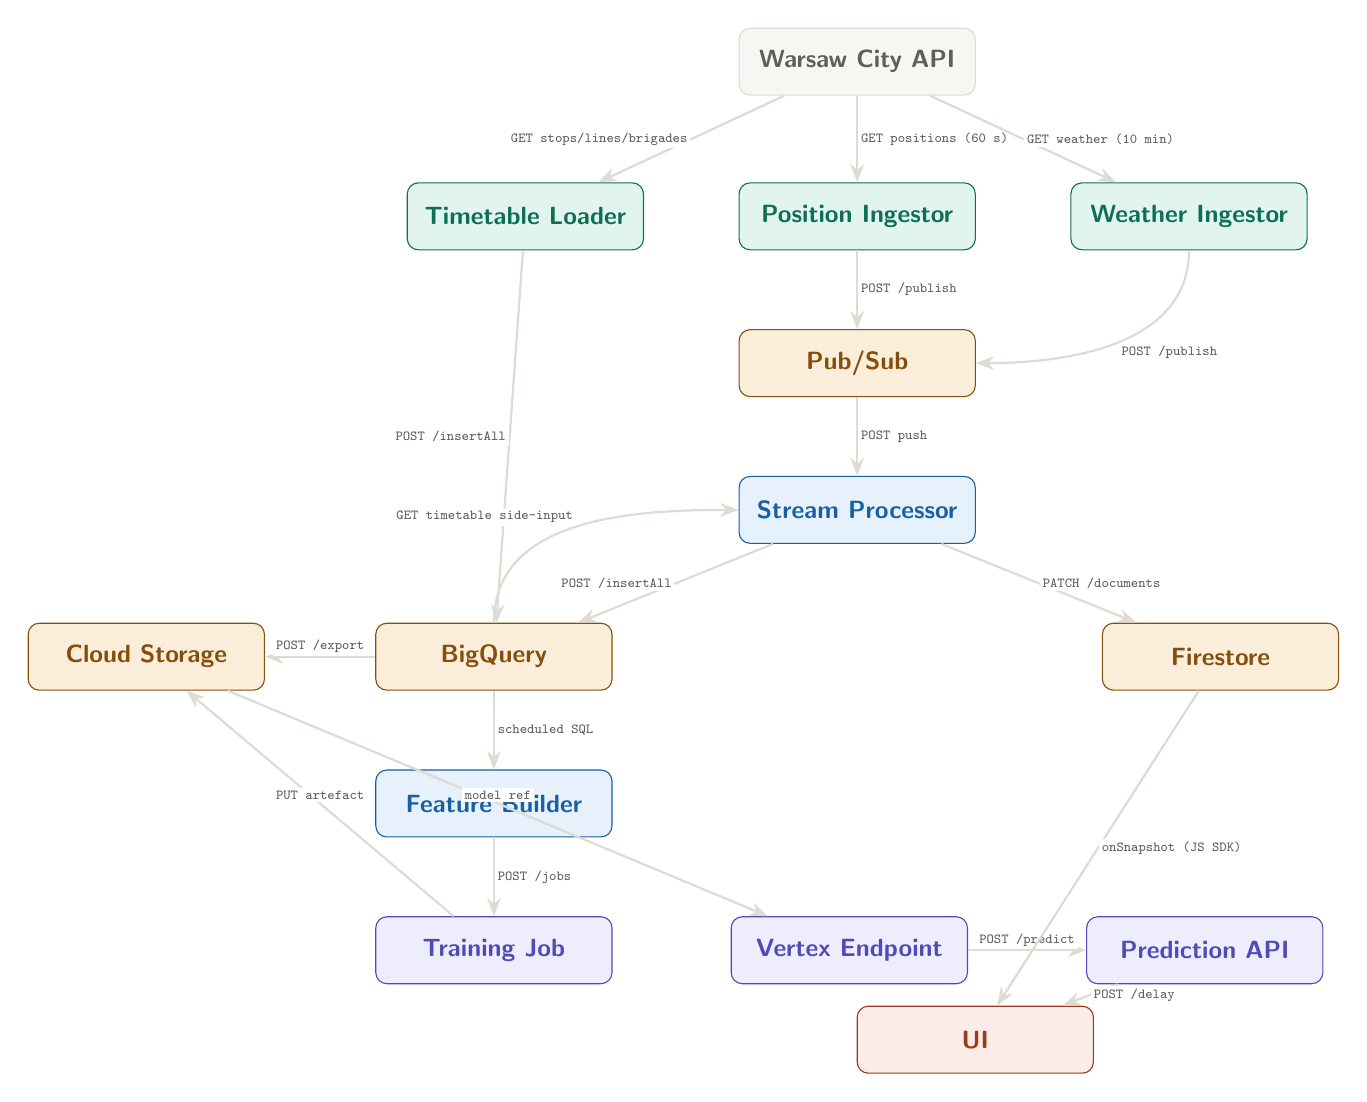
\begin{tikzpicture}[node distance=0.9cm and 1.6cm]

  % ── Row 0: external ──────────────────────────────────────────────────────
  \node[extapi] (wapi) {Warsaw City API};

  % ── Row 1: ingestors ─────────────────────────────────────────────────────
  \node[ingestion, below left=1.1cm and 1.2cm of wapi]   (ttloader)  {Timetable Loader};
  \node[ingestion, below=1.1cm of wapi]                  (posingest) {Position Ingestor};
  \node[ingestion, below right=1.1cm and 1.2cm of wapi]  (wxingest)  {Weather Ingestor};

  % ── Row 2: message bus ────────────────────────────────────────────────────
  \node[storage, below=1.0cm of posingest] (pubsub) {Pub/Sub};

  % ── Row 3: stream processor ──────────────────────────────────────────────
  \node[processing, below=1.0cm of pubsub] (stream) {Stream Processor};

  % ── Row 4: storage ────────────────────────────────────────────────────────
  \node[storage, below left=1.0cm and 1.6cm of stream]  (bq)  {BigQuery};
  \node[storage, below right=1.0cm and 1.6cm of stream] (fs)  {Firestore};
  \node[storage, left=1.4cm of bq]                      (gcs) {Cloud Storage};

  % ── Row 5: ML ─────────────────────────────────────────────────────────────
  \node[processing, below=1.0cm of bq]    (feat)    {Feature Builder};
  \node[serving, below=1.0cm of feat]     (train)   {Training Job};
  \node[serving, right=1.5cm of train]    (vertex)  {Vertex Endpoint};
  \node[serving, right=1.5cm of vertex]   (predapi) {Prediction API};

  % ── Row 6: frontend ──────────────────────────────────────────────────────
  \node[frontend, below left=4.0cm and 0.1cm of fs] (fe) {UI};

  % ── Edges ────────────────────────────────────────────────────────────────
  \draw[conn] (wapi) -- node[lbl, left] {GET stops/lines/brigades} (ttloader);
  \draw[conn] (wapi) -- node[lbl, right]{GET positions (60 s)}     (posingest);
  \draw[conn] (wapi) -- node[lbl, right]{GET weather (10 min)}     (wxingest);

  \draw[conn] (ttloader) -- node[lbl, left]{POST /insertAll} (bq);

  \draw[conn] (posingest) -- node[lbl, right]{POST /publish} (pubsub);
  \draw[conn] (wxingest.south) to[out=270,in=0]
    node[lbl, below right]{POST /publish} (pubsub.east);

  \draw[conn] (pubsub) -- node[lbl, right]{POST push} (stream);

  \draw[conn] (bq.north) to[out=90,in=180]
    node[lbl, above left]{GET timetable side-input} (stream.west);

  \draw[conn] (stream) -- node[lbl, left] {POST /insertAll}  (bq);
  \draw[conn] (stream) -- node[lbl, right]{PATCH /documents} (fs);

  \draw[conn] (bq)   -- node[lbl, above]{POST /export}  (gcs);
  \draw[conn] (bq)   -- node[lbl, right]{scheduled SQL} (feat);
  \draw[conn] (feat) -- node[lbl, right]{POST /jobs}    (train);
  \draw[conn] (train)  -- node[lbl, above]{PUT artefact} (gcs);
  \draw[conn] (gcs)    -- node[lbl, above]{model ref}    (vertex);
  \draw[conn] (vertex) -- node[lbl, above]{POST /predict}(predapi);

  % Firestore → Frontend (Firestore JS SDK, direct)
  \draw[conn] (fs)      -- node[lbl, right]{onSnapshot (JS SDK)} (fe);
  % Prediction API → Frontend
  \draw[conn] (predapi) -- node[lbl, right]{POST /delay}         (fe);

\end{tikzpicture}
\caption{Microservice connection diagram.
Teal = ingestion; blue = processing; purple = ML serving;
orange = storage; coral = frontend.
The timetable BigQuery tables act as a shared side-input:
loaded once by the Timetable Loader, read continuously by the Stream Processor.
The UI reads live vehicle state directly from Firestore via the
Firestore JS SDK \texttt{onSnapshot} listener.}
\end{figure}

% =============================================================================
\section{API Design}
\label{sec:api}
% =============================================================================

\subsection{Protocol selection principles}

The default protocol for all boundaries is \textbf{REST/HTTPS with JSON
payloads}. A non-REST protocol is used only where a concrete, quantified
benefit justifies the added operational complexity. Two cases qualify
in this system; both are identified below.

\subsection{External API calls (Warsaw city API)}

All Warsaw API endpoints are polled over plain HTTP GET and return JSON.
No authentication beyond an API key in the query string is required.

\begin{table}[H]
\centering
\caption{External REST calls}
\renewcommand{\arraystretch}{1.38}
\begin{tabularx}{\linewidth}{L{3.4cm} C{1.2cm} L{2.8cm} X}
\toprule
\hd{Caller} & \hd{Method} & \hd{Endpoint (abbreviated)} & \hd{Cadence} \\
\midrule
\rowcolor{rowgray}
Timetable Loader & GET & \texttt{/dbstore\_get} (stops) & Once at 03:00 \\
Timetable Loader & GET & \texttt{/dbtimetable\_get} (lines per stop) & Once at 03:00 \\
\rowcolor{rowgray}
Timetable Loader & GET & \texttt{/dbtimetable\_get} (brigades per stop--line) & Once at 03:00 \\
Position Ingestor & GET & \texttt{/wsstore\_get} (tram positions) & Every 60 s \\
\rowcolor{rowgray}
Weather Ingestor & GET & \texttt{/imgw\_get} (Warsaw weather) & Every 10 min \\
\bottomrule
\end{tabularx}
\end{table}

\subsection{Internal service APIs}

\begin{table}[H]
\centering
\caption{Internal API contracts}
\renewcommand{\arraystretch}{1.38}
\begin{tabularx}{\linewidth}{L{3.0cm} C{2.0cm} L{3.4cm} X}
\toprule
\hd{From $\to$ To} & \hd{Protocol} & \hd{Operation} & \hd{Justification} \\
\midrule
\rowcolor{rowgray}
Timetable Loader $\to$ BigQuery
  & REST & \texttt{POST /insertAll}
  & Standard BQ streaming insert \\
Position Ingestor $\to$ Pub/Sub
  & REST & \texttt{POST /\{topic\}:publish}
  & Batch up to 1\,000 msgs \\
\rowcolor{rowgray}
Weather Ingestor $\to$ Pub/Sub
  & REST & \texttt{POST /\{topic\}:publish}
  & Same topic, different \texttt{source} attr \\
Pub/Sub $\to$ Stream Processor
  & \textbf{Pub/Sub push}$^{*}$
  & POST to Cloud Run URL
  & Managed delivery; GCP handles retries \\
\rowcolor{rowgray}
Stream Processor $\to$ BigQuery
  & REST & \texttt{POST /insertAll}
  & Micro-batched rows \\
Stream Processor $\to$ Firestore
  & REST & \texttt{PATCH /\{document\}}
  & Upsert vehicle state \\
\rowcolor{rowgray}
Stream Processor $\leftarrow$ BigQuery (side input)
  & \textbf{gRPC}$^{\dagger}$
  & BQ Storage Read API
  & See note below \\
Frontend $\to$ Firestore
  & Firestore JS SDK & \texttt{onSnapshot} listener
  & Direct browser access; push updates; no intermediate service \\
\rowcolor{rowgray}
Frontend $\to$ Prediction API
  & REST & \texttt{POST /v1/delay}
  & Request--response \\
\bottomrule
\end{tabularx}
\end{table}

\noindent
$^{*}$\textbf{Pub/Sub push vs.\ pull.}
Push delivery (GCP POSTs to the Stream Processor's Cloud Run URL) is used
rather than pull because it integrates natively with Cloud Run's concurrency
model and eliminates long-polling overhead.
This is not a separate protocol --- it is still HTTP --- but it inverts
the connection direction.

\noindent
$^{\dagger}$\textbf{gRPC for BigQuery Storage Read API.}
The Stream Processor loads the daily timetable as a Dataflow side input.
The BigQuery Storage Read API uses gRPC + Apache Arrow over the wire and
achieves \textbf{10--40$\times$ higher throughput} than the REST JSON
\texttt{tabledata.list} endpoint for bulk reads
(Google benchmark: \textasciitilde{}10 GB/s vs.\ \textasciitilde{}300 MB/s).
At daily timetable size ($\approx$50--200 MB) the difference is modest, but
this API is the standard Dataflow BigQuery source connector and requires no
additional code or schema management on our side.
It is the only gRPC surface in the system and is encapsulated inside the
Dataflow runner --- no custom Protobuf schemas are maintained by the team.

\subsection{Prediction API --- endpoint specification}

\textbf{Base URL:} \texttt{https://api.trams.warsaw/v1}

\begin{table}[H]
\centering
\caption{Prediction API endpoints}
\renewcommand{\arraystretch}{1.38}
\begin{tabularx}{\linewidth}{L{1.2cm} L{4.6cm} L{2.2cm} X}
\toprule
\hd{Method} & \hd{Path} & \hd{Auth} & \hd{Description} \\
\midrule
\rowcolor{rowgray}
POST & \texttt{/delay} & API key
  & Predict delay for a tram at a given stop and time \\
GET  & \texttt{/health} & None & Liveness probe \\
\bottomrule
\end{tabularx}
\end{table}

\textbf{POST /delay --- request:}
\begin{verbatim}
{
  "line":      "3",
  "stop_id":   "1001",
  "brigade":   "1",
  "timestamp": "2025-09-01T08:15:00Z"
}
\end{verbatim}

\textbf{POST /delay --- response:}
\begin{verbatim}
{
  "delay_seconds":  134,
  "confidence":     0.78,
  "model_version":  "v2.1.0",
  "features_used":  ["precip_mm", "route_avg_delay_30m",
                     "hour_of_day", "brigade_delay_history"]
}
\end{verbatim}

\subsection{Firestore live vehicle data}

The Frontend SPA reads live vehicle state directly from Firestore using the
Firestore JS SDK \texttt{onSnapshot} listener, receiving push updates as
documents change. Each document in the \texttt{vehicles} collection is keyed
by \texttt{vehicle\_number} and has the following shape:

\begin{verbatim}
{
  "vehicle_number": "3456",
  "line":           "3",
  "brigade":        "1",
  "lat":            52.2297,
  "lon":            21.0122,
  "delay_s":        134,
  "next_stop_id":   "1002",
  "updated":        1725174897
}
\end{verbatim}

The \texttt{updated} timestamp allows the frontend to expire vehicles not seen
for more than 120 s. Firestore security rules restrict reads to authenticated
users; no service credentials are embedded in the client bundle.

\textbf{Staleness budget.}
Warsaw API publishes positions every 60 s.
The Stream Processor adds up to 90 s of processing latency (p95).
Firestore push delivery adds negligible latency ($<$1 s).
Total end-to-end staleness: $\approx$151 s, dominated by the 60 s source
cadence --- not by any polling interval.

\section{Storage Characteristics}


\begin{table}[H]
\centering
\caption{Storage characteristics per data store}
\renewcommand{\arraystretch}{1.48}
\begin{tabularx}{\linewidth}{L{2.2cm} L{1.6cm} L{1.8cm} L{2.2cm} L{1.6cm} L{2.0cm} X}
\toprule
\hd{Store} & \hd{Structure} & \hd{SQL / NoSQL} & \hd{Consistency} & \hd{Access} & \hd{Est. volume} & \hd{Notes} \\
\midrule
\rowcolor{rowgray}
BQ timetable & Structured & SQL & Strong$^{a}$ & R \& W & 50--200 MB/day & Written once at 03:00; read-only during traffic hours \\
BQ positions (raw) & Structured & SQL & Eventual & R \& W & 3--8 GB/month & Append-only; partitioned by \texttt{date} \\
\rowcolor{rowgray}
BQ positions (enriched) & Structured & SQL & Eventual & R \& W & 5--15 GB/month & Includes \texttt{delay\_s}, next stop, weather join; training source \\
BQ features & Structured & SQL & Eventual & R \& W & 1--3 GB/month & Daily rolling aggregates; clustered on \texttt{line}, \texttt{hour} \\
\rowcolor{rowgray}
Cloud Storage & Unstructured & --- & Strong (obj) & R \& W & 50--200 MB/model & Raw JSON archive + model artefacts \\
Firestore & Semi-struct. & NoSQL (doc) & Strong (per-doc) & R \& W & $<$100 MB & Live vehicle state; TTL 2 h; read directly by frontend via JS SDK \\
\rowcolor{rowgray}
Pub/Sub & Unstructured & --- & At-least-once & W / R & $<$500 MB/month & 7-day retention; not a durable store \\
\bottomrule
\end{tabularx}
\end{table}

\noindent\small
$^{a}$ The timetable table is written once and is fully visible before
the streaming pipeline reads it.
BigQuery eventual consistency is not a concern here because
the Timetable Loader will be set to finish before the start of other reads.

\normalsize

\subsection{BigQuery dataset structure}

BigQuery holds four logical tables, all in the same dataset
\texttt{trams\_warsaw}:

\begin{description}[leftmargin=2em, style=nextline, itemsep=5pt]
  \item[\texttt{timetable}]
    Written daily at 03:00 by the Timetable Loader. Schema:
    \texttt{stop\_id}, \texttt{stop\_name}, \texttt{lat}, \texttt{lon},
    \texttt{line}, \texttt{brigade}, \texttt{scheduled\_departure} (TIMESTAMP).
    Partitioned by \texttt{load\_date}.
    \textbf{Read-only during traffic hours} --- the Stream Processor loads it
    as a Dataflow side input once at pipeline startup.

  \item[\texttt{positions\_raw}]
    Append-only. One row per GPS ping from the Warsaw API.
    Fields: \texttt{vehicle\_number}, \texttt{line}, \texttt{brigade},
    \texttt{lat}, \texttt{lon}, \texttt{gps\_time}, \texttt{ingested\_at}.
    Partitioned by \texttt{DATE(ingested\_at)}.

  \item[\texttt{positions\_enriched}]
    Computed by the Stream Processor. Extends \texttt{positions\_raw} with:
    \texttt{matched\_stop\_id}, \texttt{scheduled\_departure},
    \texttt{delay\_s}, \texttt{precip\_mm}, \texttt{temp\_c}.
    Partitioned by \texttt{DATE(gps\_time)}, clustered on \texttt{line}.
    This is the primary training input.

  \item[\texttt{features}]
    Materialised daily by the Feature Builder (BigQuery scheduled SQL).
    Rows represent (line, brigade, stop, hour-of-day) aggregates over a
    rolling 90-day window: mean delay, delay standard deviation,
    rain--delay correlation, peak-hour flag.
    Clustered on \texttt{line}, \texttt{hour\_of\_day}.
\end{description}

\subsection{Firestore}

Firestore stores only the \textbf{current operational state}: one document
per active tram, keyed by \texttt{vehicle\_number}. Documents are overwritten
(upserted) by the Stream Processor on every position update and expire via
TTL after 2 hours of inactivity --- preventing accumulation of stale entries
for trams that have completed service.

The Frontend SPA subscribes to the \texttt{vehicles} collection via the
Firestore JS SDK \texttt{onSnapshot} listener, receiving push updates as
documents change. Firestore security rules restrict reads to authenticated
users only.

Outside traffic hours (01:00--04:00) no writes occur and the collection
drains to empty via TTL.

\subsection{Cloud Storage}

Two buckets:
\begin{itemize}[itemsep=2pt]
  \item \texttt{trams-raw-archive} --- daily JSON exports from
    \texttt{positions\_raw}; 60-day lifecycle rule then auto-delete.
  \item \texttt{trams-ml-artefacts} --- versioned model files written by the
    Training Job; never auto-deleted; referenced by the Vertex AI Endpoint.
\end{itemize}

% =============================================================================
\section{SLA, SLO and SLI}
% =============================================================================



All availability SLOs are measured \textbf{within the 04:00--01:00 traffic
window only}. Services that are legitimately idle outside this window are not
penalised for being stopped.

\subsection{Per-service SLI / SLO / SLA}

\begin{longtable}{L{2.6cm} L{4.0cm} C{1.7cm} C{1.7cm} L{2.8cm}}
\caption{SLI, SLO and SLA per service} \\
\toprule
\hd{Service} & \hd{SLI} & \hd{SLO} & \hd{SLA} & \hd{Window} \\
\midrule
\endfirsthead
\multicolumn{5}{l}{\small\itshape continued\ldots} \\[2pt]
\toprule
\hd{Service} & \hd{SLI} & \hd{SLO} & \hd{SLA} & \hd{Window} \\
\midrule
\endhead
\bottomrule
\endlastfoot

\rowcolor{rowgray}
\multirow{2}{2.6cm}{Timetable Loader}
  & Load completion before 04:00 & 99\% & 95\%
  & Daily (30-day rolling) \\
  & Full timetable row count vs.\ prior day $\pm$10\% & 99\% & 95\%
  & Per run \\[4pt]

\rowcolor{rowgray}
\multirow{2}{2.6cm}{Position Ingestor}
  & Successful poll ratio (Warsaw API non-5xx) & 95\% & 90\%
  & Rolling 24 h \\
  & Position freshness: age of newest ping in Pub/Sub & $\le$90 s & $\le$3 min
  & p99 / 1 h \\[4pt]

\rowcolor{rowgray}
\multirow{2}{2.6cm}{Stream Processor}
  & Message processing latency (push $\to$ BQ write) & $\le$90 s & $\le$3 min
  & p95 / 1 h \\
  & Pipeline availability (traffic hours) & 99.5\% & 99\%
  & Rolling 30 d \\[4pt]

\rowcolor{rowgray}
\multirow{2}{2.6cm}{Prediction API}
  & Request success rate (HTTP 2xx) & 99.5\% & 99\%
  & Rolling 7 d \\
  & Prediction latency (end-to-end) & $\le$800 ms & $\le$2 s
  & p95 / h \\[4pt]

\rowcolor{rowgray}
\multirow{1}{2.6cm}{Training Job}
  & Age of deployed model & $\le$7 d & $\le$14 d
  & Continuous \\[4pt]

\rowcolor{rowgray}
\multirow{2}{2.6cm}{Frontend SPA}
  & Page load time (LCP) & $\le$2.5 s & $\le$4 s
  & p75 / 24 h \\
  & Availability (Firebase Hosting) & 99.9\% & 99.5\%
  & Rolling 30 d \\

\end{longtable}

\subsection{Error budgets (30-day traffic-hours window)}

\begin{table}[H]
\centering
\caption{Monthly error budgets}
\renewcommand{\arraystretch}{1.38}
\begin{tabularx}{\linewidth}{L{3.6cm} C{2.0cm} C{2.4cm} X}
\toprule
\hd{Service / SLI} & \hd{SLO} & \hd{Budget (min/month)} & \hd{Notes} \\
\midrule
\rowcolor{rowgray}
Stream Processor availability & 99.5\% & 189 min & $\approx$3.1 h/month at 21 h/day \\
Prediction API success rate & 99.5\% & 189 min & Vertex cold-start main risk \\
\rowcolor{rowgray}
Frontend availability & 99.9\% & 38 min & Firebase SLA covers most of this \\
\bottomrule
\end{tabularx}
\end{table}

\noindent\small\textit{Budgets are computed over the 21-hour traffic window only
($30 \times 21 \times 60 = 37\,800$ minutes/month), not the full calendar month.}

\normalsize

\subsection{Timetable Loader risk}

The Timetable Loader must complete within the 03:00--04:00 window (60 min).
If it overruns or fails, the Stream Processor starts with a stale timetable
(yesterday's), which is acceptable for most days but will produce incorrect
delays on days when the schedule changes significantly (e.g.\ first day after
a timetable revision). Mitigations:

\begin{enumerate}[itemsep=2pt]
  \item Loader writes a \texttt{load\_status} document to Firestore on
    completion; the Stream Processor checks this at startup and emits a
    Cloud Monitoring alert if the timetable is more than 26 hours old.
  \item Bounded async concurrency (40 workers) keeps wall-clock load time
    under 20 minutes, leaving 40 minutes of margin.
  \item On failure, Cloud Run Job retries automatically (max 3 attempts).
\end{enumerate}

\subsection{Vertex AI cold-start risk}

With \texttt{min-replica-count: 0}, a Vertex Endpoint cold start takes
25--45 s, breaching the p95 800 ms SLO. Mitigation options in order of cost:

\begin{enumerate}[itemsep=2pt]
  \item \texttt{min-replica-count: 1} during 04:00--01:00 via Cloud Scheduler
    toggle --- adds \$15--25/month.
  \item Cache common (line, stop, hour) predictions in Cloud Memorystore
    (Redis) --- eliminates most cold starts at \$10/month.
  \item Accept the SLO breach and commit the SLA to p95 $\le$2 s,
    which cold starts satisfy.
\end{enumerate}


\section{Summary}

\begin{table}[H]
\centering
\caption{Architecture decision summary}
\renewcommand{\arraystretch}{1.38}
\begin{tabularx}{\linewidth}{L{3.4cm} X}
\toprule
\hd{Dimension} & \hd{Decision} \\
\midrule
\rowcolor{rowgray}
Scope & Trams only; 04:00--01:00 operating window \\
Data sources & Warsaw city API only (timetable, positions, weather) \\
\rowcolor{rowgray}
Timetable ingestion
  & 3-level sequential--parallel hierarchy (stops $\to$ lines $\to$ brigades);
    written to BQ before 04:00 daily \\
Delay computation
  & Computed on our side by matching GPS positions to the loaded timetable;
    no ZTM-side delay feed exists \\
\rowcolor{rowgray}
API protocols
  & REST/HTTPS default; gRPC used only for BQ Storage Read API
    (Dataflow built-in, no team-owned schema);
    Firestore JS SDK for frontend live data \\
Primary storage
  & BigQuery (timetable + enriched positions + features) +
    Firestore (live vehicle state, read directly by frontend via JS SDK) \\
\rowcolor{rowgray}
ML platform & Vertex AI Training + Vertex AI Endpoint; artefacts in GCS \\
Cost strategy & Scale-to-zero on all Cloud Run services;
    partitioned/clustered BQ; no always-on GPU \\

\bottomrule
\end{tabularx}
\end{table}

\vfill
\begin{center}
\small\color{textmuted}
Warsaw Tram Delay Prediction Platform \textperiodcentered{}
Architecture Report \textperiodcentered{} \today
\end{center}

\end{document}